\documentclass[a4paper,14pt]{extarticle}
\usepackage{polyglossia}
\setmainlanguage{english}
\setotherlanguage{russian}
\setmainfont{DXLubava}
\usepackage{amssymb,amsfonts,amsmath,cite,enumerate,float,indentfirst}
\usepackage{geometry} % Меняем поля страницы
\geometry{left=2cm}% левое поле
\geometry{right=1.5cm}% правое поле
\geometry{top=1cm}% верхнее поле
\geometry{bottom=2cm}% нижнее поле
\usepackage{graphicx}
\graphicspath{{pic1/}}
\renewcommand{\theenumi}{\arabic{enumi}}% Меняем везде перечисления на цифра.цифра
\renewcommand{\labelenumi}{\arabic{enumi}}% Меняем везде перечисления на цифра.цифра
\renewcommand{\theenumii}{.\arabic{enumii}}% Меняем везде перечисления на цифра.цифра
\renewcommand{\labelenumii}{\arabic{enumi}.\arabic{enumii}.}% Меняем везде перечисления на цифра.цифра
\renewcommand{\theenumiii}{.\arabic{enumiii}}% Меняем везде перечисления на цифра.цифра
\renewcommand{\labelenumiii}{\arabic{enumi}.\arabic{enumii}.\arabic{enumiii}.}% Меняем везде перечисления на цифра.цифра

\usepackage{caption}
\usepackage{color}
\usepackage{xcolor}
\usepackage{listings}

\newcommand{\imgh}[3]
{
\begin{figure}[h]
    \center{\includegraphics[width=#1]{#2}}
    \caption{#3}
    \label{ris:#2}
\end{figure}
}

\begin{document}
    \begin{titlepage}
	\newpage
	
	\begin{center}
		Университет ИТМО \\
	\end{center}
	
	\vspace{1em}
	
	\begin{center}
		\Large Кафедра Мехатроники \\ 
	\end{center}
	
	\vspace{8em}
	
	\begin{center}
		\textsc{\textbf{Курсовой проект:\linebreak \newline \huge "НАЗВАНИЕ КУРСОВОГО ПРОЕКТА}}
	\end{center}
	
	\vspace{14em}
\begin{flushright}
	\begin{tabular}{rl}
		Преподаватель: & Д.В. Куприянов \\
		Выполнили: & Иван Иванов  \\
		&  Пётр Петров \\
		&  Сидор Сидоров \\
		Группа: & P4444\\
	\end{tabular}
\end{flushright}
	

	
	
	\vspace{\fill}
	
	\begin{center}
		Санкт-Петербург \\2017
	\end{center}
	
\end{titlepage}% это титульный лист
    \newpage
    \tableofcontents
    
	\newpage
	
	\begin{center}	
		\section{Введение}
		
		\end{center}
\subsection{Описание проекта}
Что же сделано?
\subsection{Актуальность}
Зачем оно нужно?
\subsection{Цель работы}
Каким образом и что нового было изучено?
    	\newpage
		\begin{center}	
		\section{Подготовка к работе}
			\end{center}
		\subsection{Проведение опроса об актуальности }
	Если нужно
		
		\subsection{Принципы работы составных элементов системы}
	Если нужно
	
	\begin{figure}[H] 
		\center 
		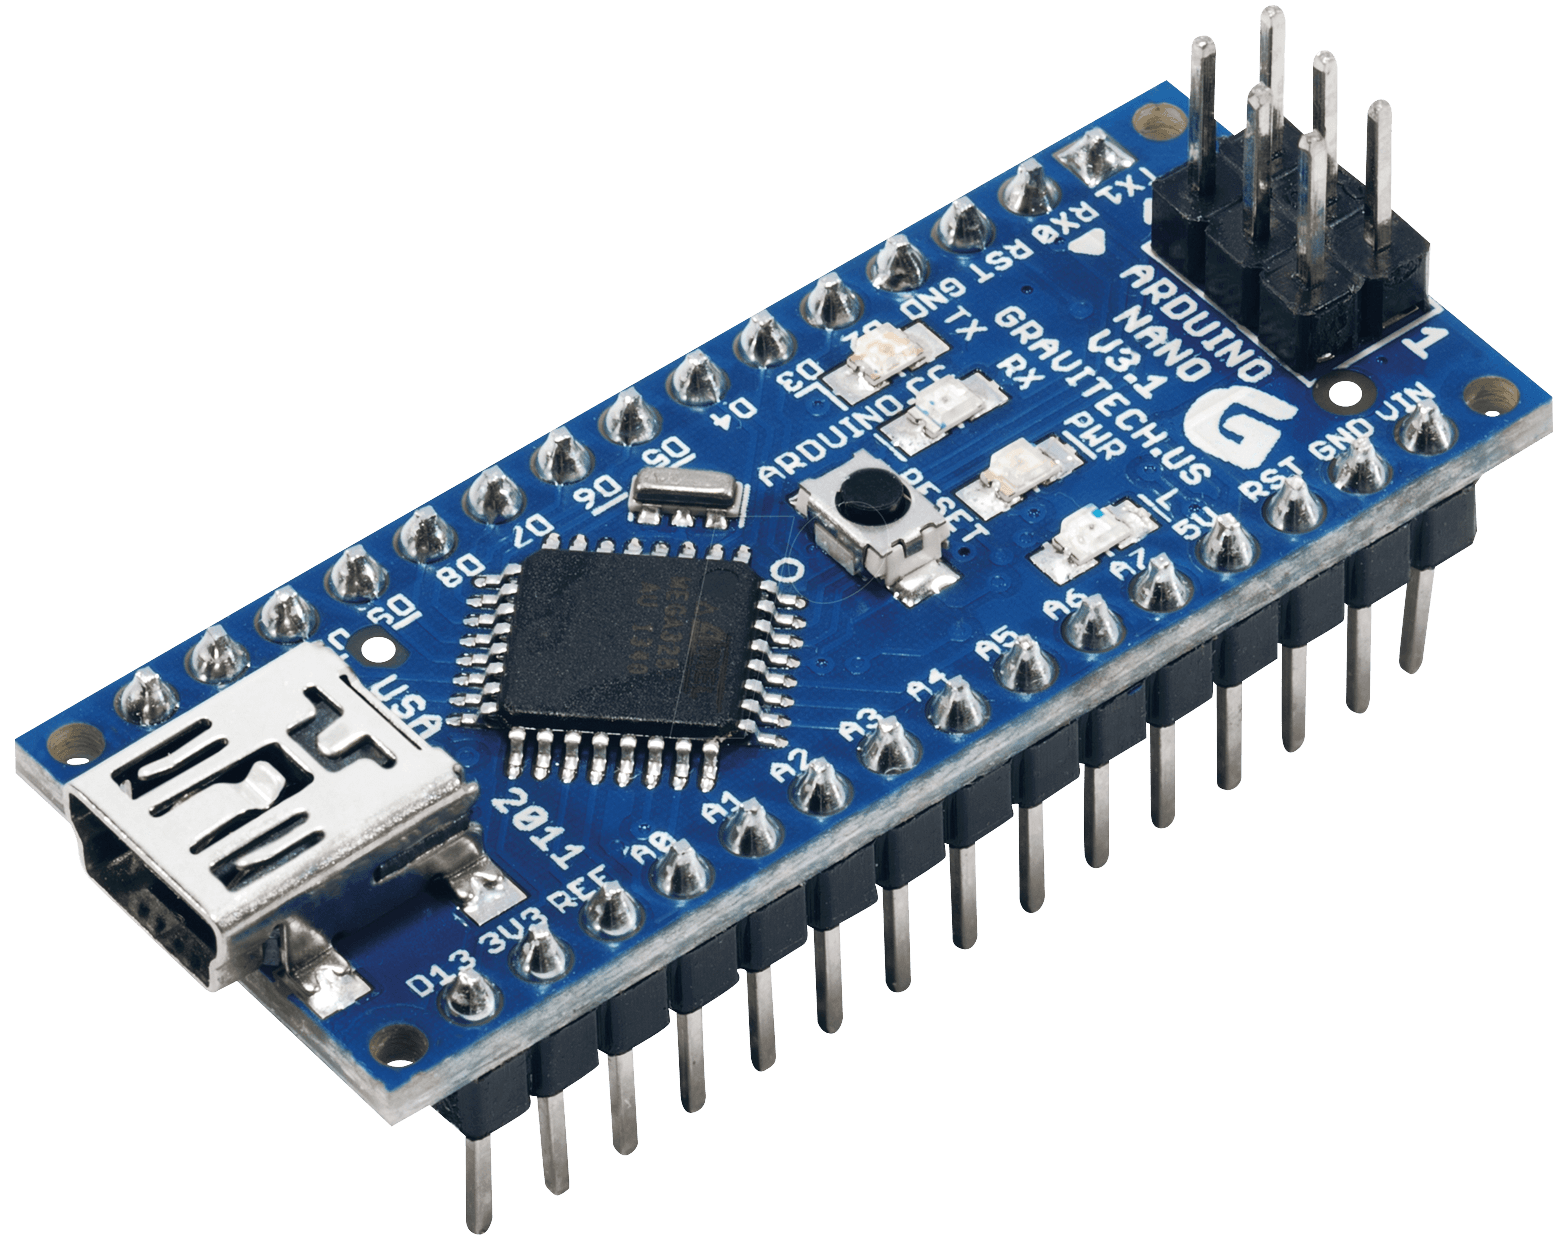
\includegraphics[width=0.7\linewidth]{principle.png} %тут в конце адрес картинки
		\caption{Текст под картинкой} 
		\label{image:principle}   %% внутренняя ссылка на картинку в рамках документа
	\end{figure}
	 В работы был использован элемент (рис.\ref{image:principle}),.
	

    
	\newpage
		\begin{center}	
				\section{Выбор комплектующих. Разработка корпуса}
		\end{center}
		\subsection{Выбор комплектующих}
	Текст 
		\newline

	
		\subsection{Разработка корпуса}
		

   
		 
		
    \newpage
		\begin{center}	
				\section{Схема подключения компонентов}
		\end{center}
	\subsection{Подключение}

\subsection{Особенность чего-то}

    \newpage
		\begin{center}	
				\section{Программный код мультиключа}
		\end{center}
    	\subsection{Описание алгоритма}
    Описание.
    	\newline
    	\newline
    	Полный код прикреплён в приложении \ref{some-code}.
    	
    
	
	
    \newpage
\begin{center}
	\section{Заключение}
	\end{center}

\subsection{Конечный результат. Итоги работы}

 Текст
	\newline
	\newline
Текст
	\newline
	\newline
Текст
	\newline
	\newline
Вывод
    \newpage

\addcontentsline{toc}{section}{Список используемой литературы}

%далее сам список используевой литературы
\begin{thebibliography}{}
	\bibitem{litlink1}  geektimes.ru/post/258674/  -  "Домофонный мультиключ и всё про имитацию «таблеток»"
	\bibitem{litlink2}  robocraft.ru/blog/arduino/82.html  -  "Программирование Arduino - EEPROM"
	\bibitem{litlink3}  electromost.com  -  "Протокол для электронных ключей RW1990"
	\bibitem{litlink4}  soltau.ru  -  "Инструкция по чтению и записи ключа iButton (1-wire) с помощью Arduino"
	\bibitem{litlink5}  easyelectronics.ru -  "Работа в Eagle Cad"
\end{thebibliography}



    \newpage

\addcontentsline{toc}{section}{Приложение}

\begin{center}
    \huge    Приложение
\end{center}

\begin{minted}{python}
def function(arg1, arg2="stroka", *, arg3=5, **kwargs):
    return arg1 + arg2 + arg3 + kwargs["arg4"]
\end{minted}



\end{document}
